\documentclass{beamer}
\usepackage[utf8]{inputenc}
\usepackage[ngerman]{babel}

\title{Kitovu %\\[1em]
	%
\includegraphics[width=8em]{../../img/logo/kitovu.jpg}
}
\subtitle{Engineering-Projekt FS 2018}
\author{Florian Bruhin \and Méline Sieber \and Nicolas Ganz}
\institute{HSR Hochschule für Technik Rapperswil}
\date{30. Mai 2018}

\begin{document}
  \frame{\titlepage}

  \begin{frame}
    \frametitle{Das Problem}
    % Ausgangsproblem: Files synchronisieren, schwierig, Florian Bruhin
    % Bisheriges: eigene Skripte (rsync), von Hand (mühsam), OpenHSR Connect (schwierig zum handhaben) - und: Moodle moosam Florian Bruhin
  \end{frame} 

  \begin{frame}
    \frametitle{Unsere Lösung: Kitovu}
    \begin{center}
    
\includegraphics[width=0.5\linewidth]{../../img/logo/kitovu.jpg}
    % Unsere Lösung: Kitovu-Logo zeigen - künstlicher Intelligenz-Tofu (haha), Worterklärung, was unser Tool kann Méline Sieber
    \end{center}
  \end{frame} 

  \begin{frame}
    \frametitle{Kitovu im Kontext}
    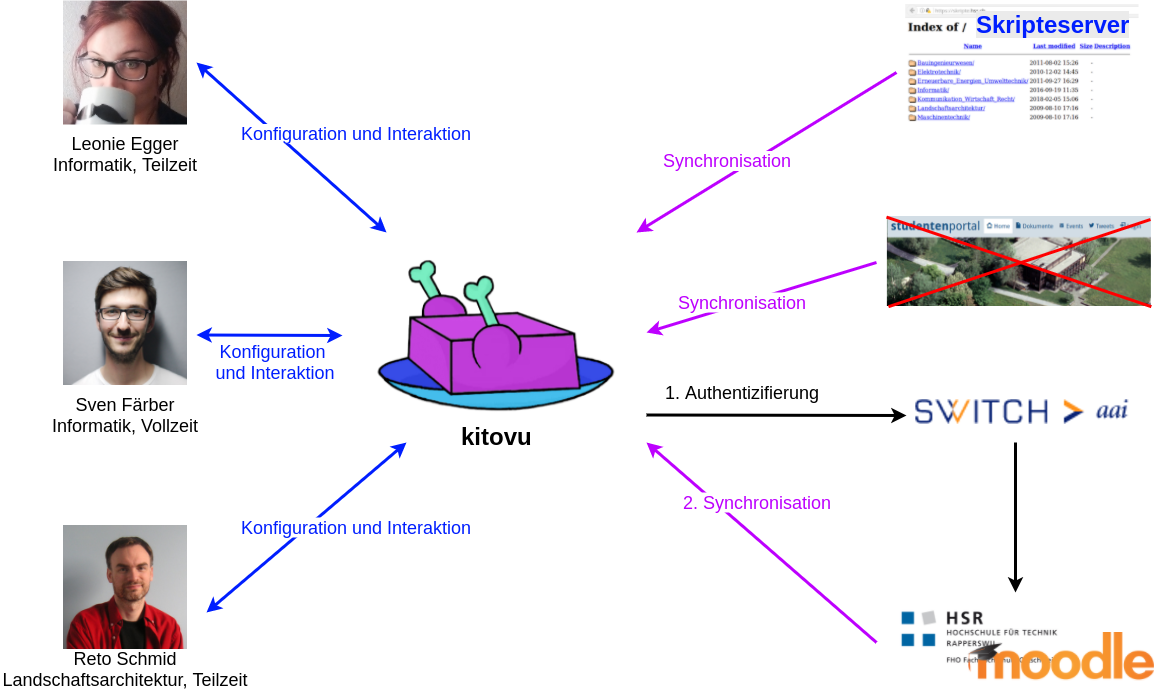
\includegraphics[width=\linewidth]{../03_End_of_Elaboration/img/kontextdiagramm.png}
    % Kontextdiagramm: Personas erklären, dann Funktionalität von Kitovu erklären Méline Sieber
  \end{frame}

  \begin{frame}
    \frametitle{Demo}
    Live-Demo...
    % Demo: 2x synchronisieren (Demo mit CLI, GUI sekundär deswegen als Zweites zeigen), Performance Nicolas Ganz
  \end{frame}

  \begin{frame}
    \frametitle{Kitovu ist plattformunabhängig}
    % Plattformunabhängigkeit: Dahinterliegende Technologie: Python, was ist SMB, PySMB Nicolas Ganz
    % Idee Flo: Ev. Logos von Python und Qt?
  \end{frame}

  \begin{frame}
    \frametitle{Kitovu ist erweiterbar}
    % Kontextdiagramm: Erweiterbarkeit wichtig => Plugin-Architektur Florian Bruhin
    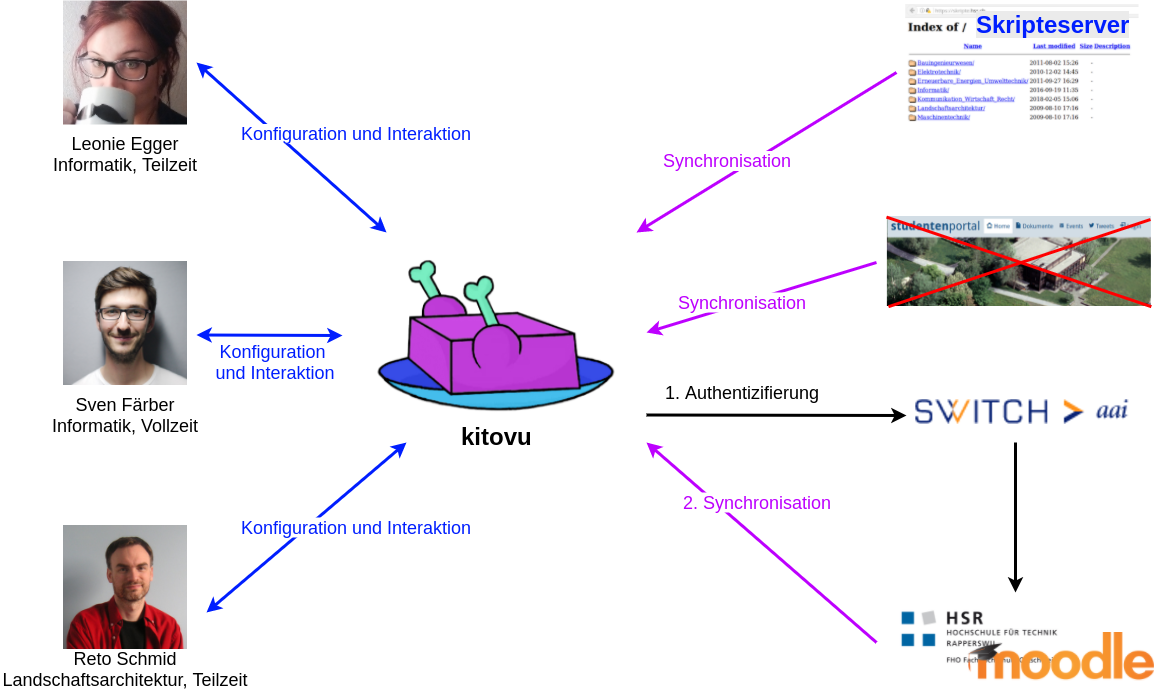
\includegraphics[width=\linewidth]{../03_End_of_Elaboration/img/kontextdiagramm.png}
  \end{frame}

  \begin{frame}
    \frametitle{Kitovu ist erweiterbar}
    % FIXME ist ggf. etwas zu überladen für ne Folie
    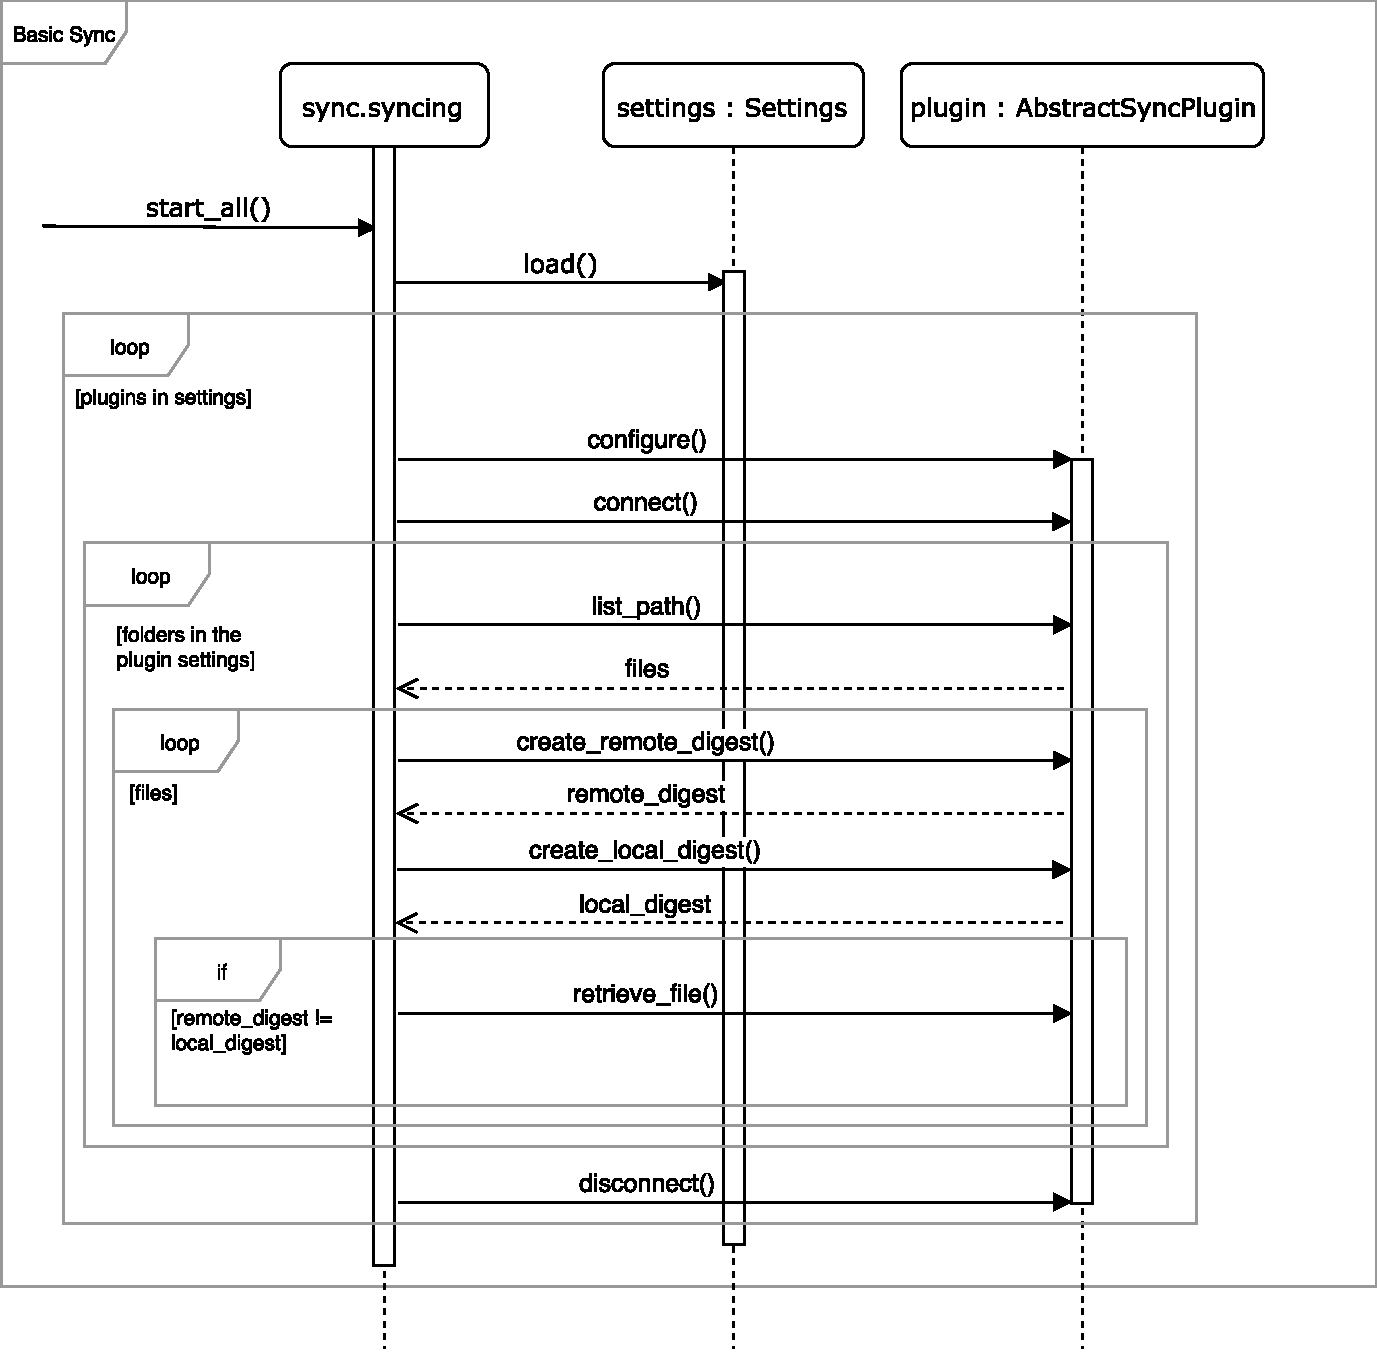
\includegraphics[height=0.9\textheight]{../03_End_of_Elaboration/img/GrobesSequenzDiagramm.pdf}
  \end{frame}

  \begin{frame}
    \frametitle{Unser Workflow}
    % Workflow: Github, Jira, Travis/Appveyor; Tools: Mypy (Typing), Pylint/Flake8, Pytest Florian Bruhin
  \end{frame}

  \begin{frame}
    \frametitle{Projektumfang}
    % Umfang/Aufwand: kleines Projekt (weil Lerneffekt, Fokus Softwareentwicklungsablauf), hat sich gelohnt nicht zu hoch zu zielen, Zeitaufwand; Klassen Méline Sieber
  \end{frame}

  \begin{frame}
    \frametitle{Fazit und Erfahrungen}
    % Fazit & Erfahrungen (3 Erfahungsberichte) Méline Sieber Gesamt: Moodle war grösste Überraschung, Studentenportal grösste Enttäuschung. Allergrösste Überraschung: alles reibungslos <3, Pair Programming super nützlich, Code Reviews, persönliche Kommunikation total wichtig (Meetings)
    % persönliche Erfahrungsberichte Méline Sieber / Nicolas Ganz / Florian Bruhin
  \end{frame}

  \begin{frame}
    \frametitle{Kitovu lebt weiter}
    % Ausblick: schönere GUI machen => Usability hat das gezeigt, Release für HSR-Studis, Sommerprojekt Nicolas Ganz
  \end{frame}

  \begin{frame}
    \frametitle{Kontakt}
    \begin{itemize}
      \item Florian Bruhin \\ \url{florian.bruhin@hsr.ch} \\[2em]
      \item Méline Sieber \\ \url{meline.sieber@hsr.ch} \\[2em]
	    \item Nicolas Ganz \\ \url{nicolas.ganz@hsr.ch} 
    \end{itemize}
  \end{frame}
  
\end{document}
